\documentclass[a4paper,english,12pt]{article}
\usepackage{%
	amsfonts,%
	amsmath,%	
	amssymb,%
	amsthm,%
	algorithm,%
	babel,%
	bbm,%
	etex,%
	%biblatex,%
	caption,%
	centernot,%
	color,%
	dsfont,%
	enumerate,%
	epsfig,%
	epstopdf,%
	geometry,%
	graphicx,%
	hyperref,%
	latexsym,%
	mathtools,%
	multicol,%
	pgf,%
	pgfplots,%
	pgfplotstable,%
	pgfpages,%
	proof,%
	psfrag,%
	subfigure,%	
	tikz,%
	ulem,%
	url%
}	
\usepackage[noend]{algpseudocode}
\usepackage[mathscr]{eucal}
\usepgflibrary{shapes}
\usetikzlibrary{%
  	arrows,%
	backgrounds,%
	chains,%
	decorations.pathmorphing,% /pgf/decoration/random steps | erste Graphik
	decorations.text,%
	matrix,%
  	positioning,% wg. " of "
  	fit,%
	patterns,%
  	petri,%
	plotmarks,%
  	scopes,%
	shadows,%
  	shapes.misc,% wg. rounded rectangle
  	shapes.arrows,%
	shapes.callouts,%
  	shapes%
}

\theoremstyle{plain}
\newtheorem{thm}{Theorem}[section]
\newtheorem{lem}[thm]{Lemma}
\newtheorem{prop}[thm]{Proposition}
\newtheorem{cor}[thm]{Corollary}

\theoremstyle{definition}
\newtheorem{defn}[thm]{Definition}
\newtheorem{conj}[thm]{Conjecture}
\newtheorem{exmp}[thm]{Example}
\newtheorem{assum}[thm]{Assumptions}
\newtheorem{axiom}[thm]{Axiom}

\theoremstyle{remark}
\newtheorem{rem}{Remark}
\newtheorem{note}{Note}
\newtheorem{fact}{Fact}

\newcommand{\norm}[1]{\left\lVert#1\right\rVert}
\newcommand{\indep}{\!\perp\!\!\!\perp}
\DeclarePairedDelimiter\abs{\lvert}{\rvert}%
\newcommand\numberthis{\addtocounter{equation}{1}\tag{\theequation}}
\newcommand{\tr}{\operatorname{tr}}
\newcommand{\R}{\mathbb{R}}
\newcommand{\N}{\mathbb{N}}
\newcommand{\E}{\mathbb{E}}
\newcommand{\Z}{\mathbb{Z}}
\newcommand{\B}{\mathscr{B}}
\newcommand{\C}{\mathcal{C}}
\newcommand{\T}{\mathscr{T}}
\newcommand{\F}{\mathcal{F}}
\newcommand{\G}{\mathcal{G}}
%\newcommand{\ba}{\begin{align*}}
%\newcommand{\ea}{\end{align*}}
\DeclareMathOperator*{\argmax}{arg\,max}
\renewcommand{\qedsymbol}{$\blacksquare$}
\makeatletter
\def\BState{\State\hskip-\ALG@thistlm}
\makeatother

\makeatletter
\def\th@plain{%
  \thm@notefont{}% same as heading font
  \itshape % body font
}
\def\th@definition{%
  \thm@notefont{}% same as heading font
  \normalfont % body font
}
\makeatother
\date{}
\title{14: Detector Performance Analysis Techniques}
\date{25 feb 2016}
\author{}
\begin{document}
\maketitle
\maketitle
In the previous lecture, quadratic detector performance analysis was done. In this lecture, we wil look at some detector performance analysis techniques. we wil see Chernoff Bound technique and look upon Markov's inequality and Jensen's inequality.
\section{Detector performance analysis techniques:}
Let us consider likelihood ratio tests(LRTs)the following example of a composite hypothesis testing problem.
\begin{eqnarray}
\tilde{\delta}(\bar{y}) &=&
\begin{cases}
1, &if~ T(\bar{y}) > \tau'.\\
\gamma, &if~  T(\bar{y}) = \tau'.\\
0, &if~ T(\bar{y}) < \tau'.\\
\end{cases}
\end{eqnarray}
Where $T: \Gamma\rightarrow\mathbb{R}$ is any function.
Detection performance typically is a function of two matrices:
\begin{eqnarray}
P_F(\tilde\delta_T) &=& P_0[T(y)>\tau]+\gamma\cdot P_0[T(y)=\tau]\\
P_M(\tilde\delta_T) &=& P_1[T(y)<\tau]+(1-\gamma)\cdot P_1[T(y)=\tau]\\
&=& 1-P_D(\tilde\delta_T)
\end{eqnarray}
Where $P_F(\tilde{\delta_T})$ is probability of false alarm and $P_M(\tilde{\delta_T})$ is the probability of miss.
In general,if $Y$ has a pdf $P_j$ under $H_j$,$j\in {0,1}$,then\\
\[P_F(\tilde{\delta_T})=\int\cdots\int_{\{y:T(y)>\tau\} \leq\Gamma(\gamma)} (P_0(y_1\cdots y_n)\cdot dy_1\cdots dy_n)\]\\
 which is typically impossible to exactly compute in closed form.As the dimension of Y increases,this integral becomes harder. 
 \subsection{Chernoff Bound technique:}
 \textbf{Markov's inequality:}If $X \geq 0$ is a random variable,r,then\\
 \[P[X\geq a]\leq \frac{\mathbb{E}[X]}{a},\forall a>0\]\\
 This helps to map probability calculations to expectation calculations which are easier than former.\\
 \textbf{Jensen's inequality:}If X is a random variable and $f:\mathbb{R}\rightarrow \mathbb{R}$ is a convex function,then
\[f(\mathbb{E})\leq \mathbf{E}[f(x)]\]
\textbf{Convex function:}
\[f[\lambda\cdot x+(1-\lambda)\cdot y]\ \leq\ \lambda\cdot f(x)+(1-\lambda)\cdot f(y),\ \forall x,y\in\mathbb{R},\ \forall \lambda \in [0,1]\]
now consider:\\
\[P_F(\tilde\delta_T)\ \leq\ P_0[T(Y)\geq\tau]\]
RHS can be written as,\\
\[P_0[s\cdot T(Y)\geq s\cdot\tau]=P_0[e^{s\cdot T(Y)}\geq e^{s\cdot\tau}],\forall s\geq 0\]
now both $e^{s\cdot T(Y)}$ and $e^{s\cdot\tau}$ are positive,so Markov's inequality can be applied.
hence,\\
\[P_0[e^{s\cdot T(Y)}\geq e^{s\cdot\tau}] \leq e^{-s\cdot\tau}\cdot\mathbb{E_0}[e^{s\cdot T(Y)}],\forall s\geq 0\]\\
RHS can be written as,
\begin{align}
e^{-s\cdot\tau+\log(\mathbb{E_0}[e^{s\cdot T(Y)}])}
= e^{-s\cdot\tau+\mu_{T,0}(S)},\forall s\geq 0
\end{align}
$\log(\mathbb{E_0}[e^{s\cdot T(Y)}])$ is the log MGF of T(Y) (Cumulant Generating Function of T at s>0).\\
Similarly,for probability for miss,
\begin{align}
&P_M(\tilde\delta_T)\leq P_1[T(Y)\leq\tau]\\
\Rightarrow &P_M(\tilde\delta_T)\leq e^{-t\cdot\tau +\mu_{T,1}(t)},\forall t<0
 \end{align}
Hence,we can choose $s>0,t<0$ to minimize the RHS in equation 5 and 7 to obtain the best bound,provided CGFs of T are known.\\
Lets look at LRTs,where
\begin{align*}
T(y)&=\log(L(y))\\
&=\log\left(\frac{P_1(y)}{P_0(y)}\right)\\
\end{align*}
here,we are comparing the above with a threshold $\tau$ ,therefore the performance of a detector is a function of $\tau$ and $T(y)$.\\
Now,from the definition of $\mu_{T,0}(s)$ and expression for $\mathbb{E}[.]$
\begin{align*}
 \mu_{T,0}(s)&=\log\left(\int_{\Gamma}{e^{s\cdot\log(L(y))}\cdot P_0(y)}\cdot dy\right)\\
&= \log\left(\int_{\Gamma}{(L(y))^s\cdot P_0(y)}\cdot dy\right)\\
\end{align*}
\begin{align*}
\mu_{T,1}(t)&=\log\left(\int_{\Gamma}{(L(y))^t\cdot \frac{P_1(y)}{P_0(y)}\cdot P_0(y)}\cdot dy\right)\\
&= \log\left(\int_{\Gamma}{(L(y))^(t+1)\cdot P_0(y)}\cdot dy\right)\\
&=\mu{T,0}(t+1)\\
\end{align*}
We are trying to bound it such that it increases by s from one side and decreases by $(t+1)$ from other(as t is negative).\\
Therefore, we have the bounds as,
\begin{align*}
&P_F(\tilde\delta_T)\leq e^{-s\cdot\tau+\mu_{T,0}(s)},\forall s\geq 0\\
&P_M(\tilde\delta_T)\leq e^{(1-s)\cdot\tau +\mu_{T,0}(s)},\forall s<1\\
\end{align*}
We get the best bound when RHS of both are minimum.RHS of both the terms are similar,except for $e^\tau$ term in second expression.\\
\large \textbf{FACTS:}
\begin{enumerate}
\item $f(s)=\mu_{T,0}(s)-s\cdot \tau$ is a convex function over s.This implies that  if,$\mu^\prime_{T,0}(s_0)=\tau,\forall s_0\forall s_0$ ,then f has a minimum at $s_0$,i.e.,$f(s)$ has its derivative zero at $s_0$.\\But if $s_0$ lies between 0 and 1,our problem of finding optimum solution will be solved,as it minimizes both the equations.Hence,$s_0$ is a global minimum and not local minimum.
\item $\mu^\prime_{T,0} (j)=\mathbb{E_j}[\log(L(y))],\forall j\in \{0,1\}$
\item $f(s)=\mu{T,0}(s)-s\cdot\tau$ is convex.\\This implies that$\mu^\prime_{T,0}(s)$is a non decreasing function of s.
\end{enumerate}
\begin{align*}
let \mu_0 &= \mu^\prime_{T,0}(0)\\&=\mathbb{E_0}[\log(L(y))]\\
&=\mathbb{E_0}\left[\log\left(\frac{P_1(y)}{P_0(y)}\right)\right]\\
\end{align*}
now,from jensen's inequality,log is a concave function,so
\begin{equation*}
\mathbb{E_0}\left[\log\left(\frac{P_1(y)}{P_0(y)}\right)\right]\leq\log\left(\mathbb{E}\left[\frac{P_1(y)}{P_0(y)}\right]\right)\\
\end{equation*}
the RHS can be written as,
\begin{align*}
\log\left(\int{\frac{P_1(y)}{P_0(y)}\cdot P_0(y) }\cdot dy\right)
&=\log(1)\\
&=0
\end{align*}
it implies that\\
\[\mu^\prime{T,0}(0)\leq 0\]
similarly,
\[\mu^\prime{T,0}(1)\geq 0\]
therefore between 0 and 1,it should cross $\mu^\prime{T,0}(1)=s$,for a given s.
\begin{figure}[hbtp]
	\centering
	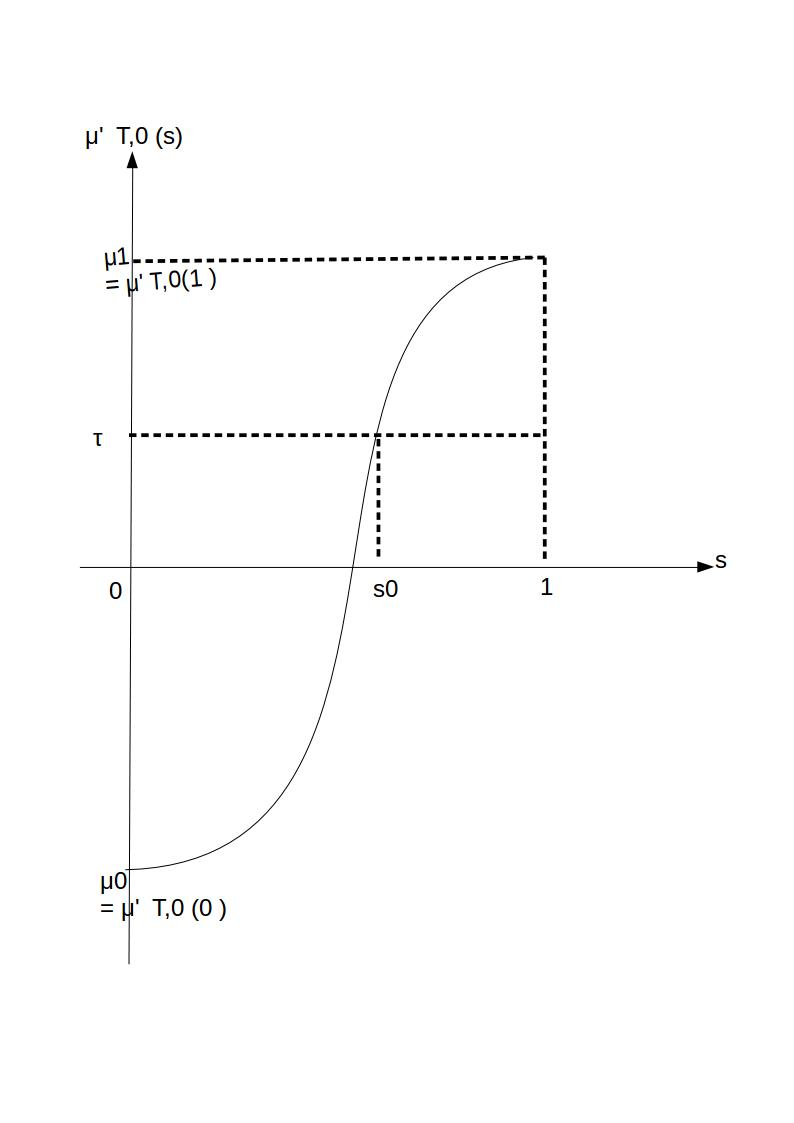
\includegraphics[scale=0.20]{Figures/Untitled1.jpg}
	\caption{variation of derivative of CGF of $T(y)$ with s.At $s_0$,$\tau$ is obtained  \\ \textit{(Source: H. Vincent Poor, An Introduction to Signal Detection and Estimation(Second Edition))}}
	\label{fn2}
\end{figure}\\
\textbf{Bottomline:}
If $\tau\in(\mu_0,\mu_1)$ then, $\exists s_0\in[0,1]:f^\prime(s_0)=0$.\\
\{KL divergence is the dual of $\log(MGF)$.therefore,$\mathbb{E_0}\left[\log\left(\frac{P_1(y)}{P_0(y)}\right)\right]$ gives a negative KL divergence.\}\\
\begin{align}
&P_F(\tilde\delta_T)\leq e^{\mu{T,0}\cdot (s_0)-s_0 \cdot \mu \prime_{T,0}(s_0)}\\
&P_M(\tilde\delta_T)\leq e^{\mu{T,0}\cdot (s_0)+(1-s_0) \cdot \mu \prime_{T,0}(s_0)}\\
\end{align}
This is called Chernoff Bound Technique.\\
\textbf{Notes:}\\
When $\tau\leq \mu_0$:
\begin{align*}
&\mu^\prime_{T,0}(s)\geq \tau,\forall s\geq 0,\\
&\Rightarrow f^\prime(s)\geq 0\\
&\Rightarrow\min_{\forall s \geq 0}{f(s)}=f(0)\\
&\Rightarrow P_F(\tilde\delta_T) \leq 1\\
\end{align*}
When$\tau\geq\mu_1:$\\
\[P_M(\tilde\delta_T)\leq 1\]
\begin{exmp}\textbf{For Bayesian hypothesis testing:}\\
assume prior probabilities are $\pi_0$ and $\pi_1$ (for $H_0$ and $H_1$) and\\
 $\pi_0 + \pi_1 = 1$ then,average probability of error,
\begin{align}
&P_e=\pi_0\cdot P_F+\pi_1\cdot P_M\\
&P_e\leq\pi_0 e^{\mu_{T,0}\cdot(s_0)-s_0\cdot \mu^\prime_{T,0}(s_0)}+\pi_1 e^{\mu_{T,0}\cdot(s_0)-(1-s_0)\cdot \mu^\prime_{T,0}(s_0)}
\end{align}
Therefore,\\
\begin{equation}
P_e\leq[\pi_0+\pi_1\cdot e^{\mu^\prime{T,0}(s_0)}]\cdot e^{\mu_{T,0}(s_0)-s_0\cdot\mu^\prime_{T,0}(s_0)}
 \end{equation}
(13) is the form of $(A+B)\cdot C$ and inequality(12)is obtained from(8)and(9).In fact, one can derive slightly tighter bound than bound obtained in (13),\\
\[P_e\leq \max\{\pi_0,\pi_1\cdot e^{\mu^\prime_{T,0}(s_0)}\}\cdot e^{\mu_{T,0}(s_0)-s_0\cdot\mu^\prime_{T,0}(s_0)},\forall 0\leq s\leq 1\]
For the detector,\[\log(L(y))\frac{>}{<}\tau\],
Recalling the minimum probability of error obtained for Bayesian decision rule assuming equal costs:\\
Choose a threshold $\tau$ such that it satisfies\\
\[Threshold, \tau=\log\left(\frac{\pi_0}{\pi_1}\right)\]
For this detector,
\begin{align*}
P_e&\leq\max\{\pi_0,\frac{\pi_0}{\pi_1}\cdot \pi_1\}\cdot e^{\mu_{T,0}(s)-s\cdot \log\left(\frac{\pi_0}{\pi_1}\right)}\\
&=\pi_0^{1-s}\cdot \pi_1^s\cdot e^{\mu_{T,0}(s)},\forall s\in [0,1]\\
\end{align*}
Therefore,\\
\[P_e\leq =\pi_0^{1-s}\cdot \pi_1^s\cdot e^{\mu_{T,0}(s)},\forall s\in [0,1]\]
Hence,one can try and optimize RHS of above equation over s.
\end{exmp}
\begin{exmp}
\textbf{IID OBSEVATIONS:}\\ 
For $\Gamma\in \mathbb{R}^n$,\\
And vector $Y=(y_1,y_2,\cdots,y_n)f_j$ under $H_j$ then,
\begin{align*}
\mu_{T,0}(s)&=\log\left(\mathbb{E_0}\left[e^{s\cdot\log(L(y))}\right]\right)\\
&=\log\left(\mathbb{E_0}\left[e^{s\cdot\log\left(\prod_{k=1}^n\frac{f_1(y_k)}{f_0(y_k)}\right)}\right]\right)\\
&=log\left(\mathbb{E_0}\left[f_1^{s}(y)\cdot f_0^{-s}(y)\right]\right)\\
&= n\cdot\log\left(\int_{\Gamma}{f_1^{s}(y)\cdot f_0^{-s}(y)\cdot f_0(y)}\cdot dy\right)\\
&= n\cdot\log\left(\int_{\Gamma}{\left[\frac{f_1(y)}{f_0(y)}\right]^{s}\cdot f_0(y)}\cdot dy \right)
\end{align*}
\begin{flushleft}
now,
\end{flushleft}
\begin{align*}\int_{\Gamma}{\left[\frac{f_1(y)}{f_0(y)}\right]^{s}\cdot f_0(y)}\cdot dy =\mathbb{E}\left[\left(\frac{f_1(y)}{f_0(y)}\right)^s\right]
\end{align*}
\begin{flushleft}
and
\end{flushleft}
\begin{align*}
\mathbb{E}\left[\left(\frac{f_1(y)}{f_0(y)}\right)^s\right]\leq\left\{\mathbb{E_0}\left[\frac{f_1(y)}{f_0(y)}\right]\right\}^s
\end{align*}
\begin{flushleft}
and we know,$\left\{\mathbb{E_0}\left[\frac{f_1(y)}{f_0(y)}\right]\right\}^s = 1$
\end{flushleft}
therefore,
\begin{align*}
\mathbb{E}\left[\left(\frac{f_1(y)}{f_0(y)}\right)^s\right] &= n\cdot \log(a),a<1\\
&= -n\cdot c,c>0 \\
\end{align*}
\end{exmp}
\textbf{Implication:}\{For minimum Probability of error for Bayesian detector\}\\
\[P_e\leq \pi_0^{1-s}\cdot \pi_1^s\cdot e^{-n\cdot c(s)},\forall s\in (0,1)\]\\
Here $c(s)$ should be positive.Probability of making an error decreases exponentially when increases. \\
\textbf{Fact:}\\
By Chernoff's theorem,optimal choice s,$s\in(0,1)$ is given by,\\
\[\max_{s\in (0,1)}{c(s)}=D(f||f_0)\]
where,$f:D(f||f_0)=D(f||f_1)$
\end{document}